\documentclass[12pt]{article}

\usepackage[top=5em, bottom=5em, left=5em, right=5em]{geometry}
\usepackage{listings}
\usepackage{tikz}
\usetikzlibrary{positioning}

\setlength\parindent{0em}
\setlength\parskip{1em}

\title {Assignment 4}

\author {Hendrik Werner s4549775}

\begin{document}
\maketitle

This was done in collaboration with Constantin Blach (s4329872).

\section{} %1
\section{} %2
We use alphabetical order as a tie breaker and begin at node $A$:

\begin{enumerate}
	\item
	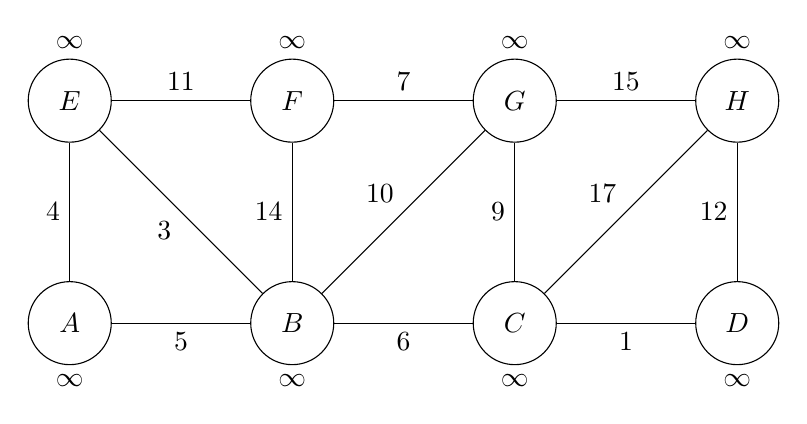
\begin{tikzpicture}[baseline=(E.north), node distance=5em ,c/.style={circle, draw, minimum width=3em}]
		\node[c] (A) {$A$};
		\node[below=0em of A] (A_label) {$\infty$};
		\node[c, right=of A] (B) {$B$};
		\node[below=0em of B] (B_label) {$\infty$};
		\node[c, right=of B] (C) {$C$};
		\node[below=0em of C] (C_label) {$\infty$};
		\node[c, right=of C] (D) {$D$};
		\node[below=0em of D] (D_label) {$\infty$};
		\node[c, above=of A] (E) {$E$};
		\node[above=0em of E] (E_label) {$\infty$};
		\node[c, above=of B] (F) {$F$};
		\node[above=0em of F] (F_label) {$\infty$};
		\node[c, above=of C] (G) {$G$};
		\node[above=0em of G] (G_label) {$\infty$};
		\node[c, above=of D] (H) {$H$};
		\node[above=0em of H] (H_label) {$\infty$};

		\path (A) edge node[below] {5} (B);
		\path (A) edge node[auto] {4} (E);
		\path (B) edge node[below] {6} (C);
		\path (B) edge node[auto] {3} (E);
		\path (B) edge node[auto] {14} (F);
		\path (B) edge node[auto] {10} (G);
		\path (C) edge node[below] {1} (D);
		\path (C) edge node[auto] {9} (G);
		\path (C) edge node[auto] {17} (H);
		\path (D) edge node[auto] {12} (H);
		\path (E) edge node[auto] {11} (F);
		\path (F) edge node[auto] {7} (G);
		\path (G) edge node[auto] {15} (H);
	\end{tikzpicture}
	\item
	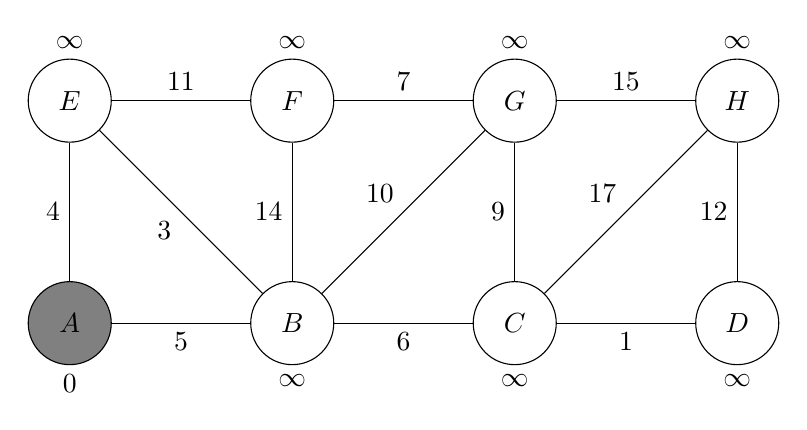
\begin{tikzpicture}[baseline=(E.north), node distance=5em ,c/.style={circle, draw, minimum width=3em}, v/.style={fill=gray}, s/.style={line width=.25em}]
		\node[c, v] (A) {$A$};
		\node[below=0em of A] (A_label) {$0$};
		\node[c, right=of A] (B) {$B$};
		\node[below=0em of B] (B_label) {$\infty$};
		\node[c, right=of B] (C) {$C$};
		\node[below=0em of C] (C_label) {$\infty$};
		\node[c, right=of C] (D) {$D$};
		\node[below=0em of D] (D_label) {$\infty$};
		\node[c, above=of A] (E) {$E$};
		\node[above=0em of E] (E_label) {$\infty$};
		\node[c, above=of B] (F) {$F$};
		\node[above=0em of F] (F_label) {$\infty$};
		\node[c, above=of C] (G) {$G$};
		\node[above=0em of G] (G_label) {$\infty$};
		\node[c, above=of D] (H) {$H$};
		\node[above=0em of H] (H_label) {$\infty$};

		\path (A) edge node[below] {5} (B);
		\path (A) edge node[auto] {4} (E);
		\path (B) edge node[below] {6} (C);
		\path (B) edge node[auto] {3} (E);
		\path (B) edge node[auto] {14} (F);
		\path (B) edge node[auto] {10} (G);
		\path (C) edge node[below] {1} (D);
		\path (C) edge node[auto] {9} (G);
		\path (C) edge node[auto] {17} (H);
		\path (D) edge node[auto] {12} (H);
		\path (E) edge node[auto] {11} (F);
		\path (F) edge node[auto] {7} (G);
		\path (G) edge node[auto] {15} (H);
	\end{tikzpicture}
	\item
	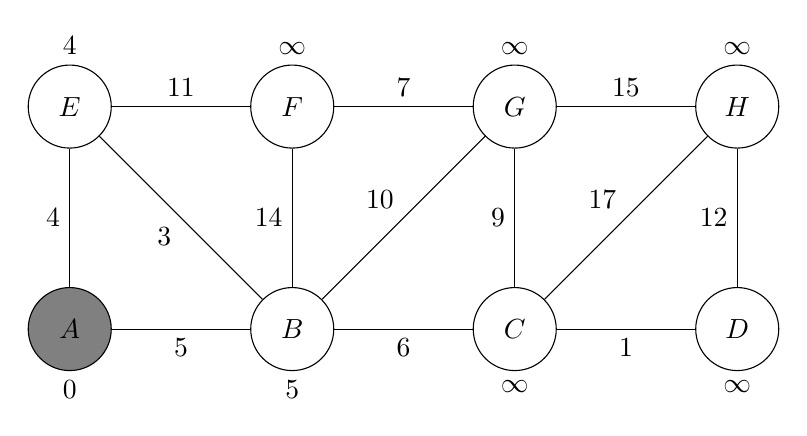
\begin{tikzpicture}[baseline=(E.north), node distance=5em ,c/.style={circle, draw, minimum width=3em}, v/.style={fill=gray}, s/.style={line width=.25em}]
		\node[c, v] (A) {$A$};
		\node[below=0em of A] (A_label) {$0$};
		\node[c, right=of A] (B) {$B$};
		\node[below=0em of B] (B_label) {$5$};
		\node[c, right=of B] (C) {$C$};
		\node[below=0em of C] (C_label) {$\infty$};
		\node[c, right=of C] (D) {$D$};
		\node[below=0em of D] (D_label) {$\infty$};
		\node[c, above=of A] (E) {$E$};
		\node[above=0em of E] (E_label) {$4$};
		\node[c, above=of B] (F) {$F$};
		\node[above=0em of F] (F_label) {$\infty$};
		\node[c, above=of C] (G) {$G$};
		\node[above=0em of G] (G_label) {$\infty$};
		\node[c, above=of D] (H) {$H$};
		\node[above=0em of H] (H_label) {$\infty$};

		\path (A) edge node[below] {5} (B);
		\path (A) edge node[auto] {4} (E);
		\path (B) edge node[below] {6} (C);
		\path (B) edge node[auto] {3} (E);
		\path (B) edge node[auto] {14} (F);
		\path (B) edge node[auto] {10} (G);
		\path (C) edge node[below] {1} (D);
		\path (C) edge node[auto] {9} (G);
		\path (C) edge node[auto] {17} (H);
		\path (D) edge node[auto] {12} (H);
		\path (E) edge node[auto] {11} (F);
		\path (F) edge node[auto] {7} (G);
		\path (G) edge node[auto] {15} (H);
	\end{tikzpicture}
	\item
	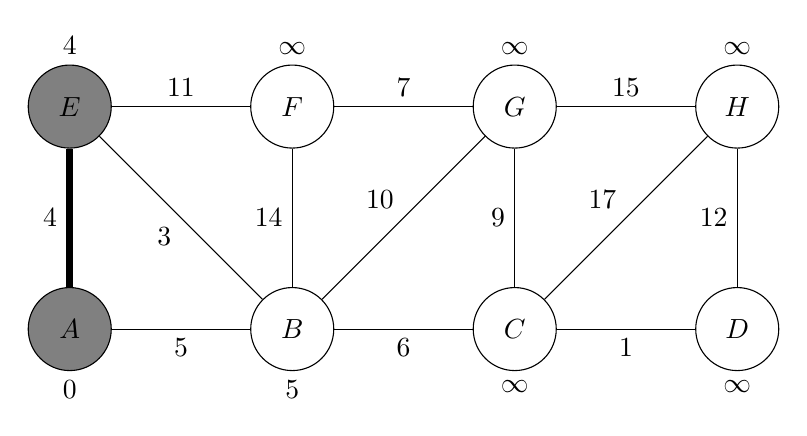
\begin{tikzpicture}[baseline=(E.north), node distance=5em ,c/.style={circle, draw, minimum width=3em}, v/.style={fill=gray}, s/.style={line width=.25em}]
		\node[c, v] (A) {$A$};
		\node[below=0em of A] (A_label) {$0$};
		\node[c, right=of A] (B) {$B$};
		\node[below=0em of B] (B_label) {$5$};
		\node[c, right=of B] (C) {$C$};
		\node[below=0em of C] (C_label) {$\infty$};
		\node[c, right=of C] (D) {$D$};
		\node[below=0em of D] (D_label) {$\infty$};
		\node[c, v, above=of A] (E) {$E$};
		\node[above=0em of E] (E_label) {$4$};
		\node[c, above=of B] (F) {$F$};
		\node[above=0em of F] (F_label) {$\infty$};
		\node[c, above=of C] (G) {$G$};
		\node[above=0em of G] (G_label) {$\infty$};
		\node[c, above=of D] (H) {$H$};
		\node[above=0em of H] (H_label) {$\infty$};

		\path (A) edge node[below] {5} (B);
		\path[s] (A) edge node[auto] {4} (E);
		\path (B) edge node[below] {6} (C);
		\path (B) edge node[auto] {3} (E);
		\path (B) edge node[auto] {14} (F);
		\path (B) edge node[auto] {10} (G);
		\path (C) edge node[below] {1} (D);
		\path (C) edge node[auto] {9} (G);
		\path (C) edge node[auto] {17} (H);
		\path (D) edge node[auto] {12} (H);
		\path (E) edge node[auto] {11} (F);
		\path (F) edge node[auto] {7} (G);
		\path (G) edge node[auto] {15} (H);
	\end{tikzpicture}
	\item
	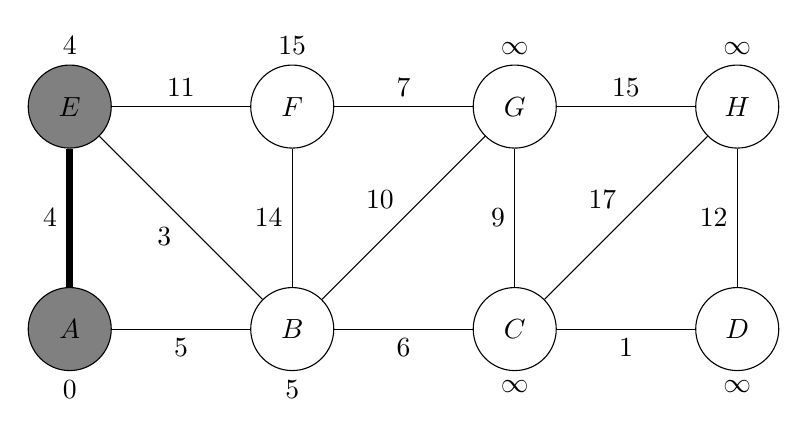
\begin{tikzpicture}[baseline=(E.north), node distance=5em ,c/.style={circle, draw, minimum width=3em}, v/.style={fill=gray}, s/.style={line width=.25em}]
		\node[c, v] (A) {$A$};
		\node[below=0em of A] (A_label) {$0$};
		\node[c, right=of A] (B) {$B$};
		\node[below=0em of B] (B_label) {$5$};
		\node[c, right=of B] (C) {$C$};
		\node[below=0em of C] (C_label) {$\infty$};
		\node[c, right=of C] (D) {$D$};
		\node[below=0em of D] (D_label) {$\infty$};
		\node[c, v, above=of A] (E) {$E$};
		\node[above=0em of E] (E_label) {$4$};
		\node[c, above=of B] (F) {$F$};
		\node[above=0em of F] (F_label) {$15$};
		\node[c, above=of C] (G) {$G$};
		\node[above=0em of G] (G_label) {$\infty$};
		\node[c, above=of D] (H) {$H$};
		\node[above=0em of H] (H_label) {$\infty$};

		\path (A) edge node[below] {5} (B);
		\path[s] (A) edge node[auto] {4} (E);
		\path (B) edge node[below] {6} (C);
		\path (B) edge node[auto] {3} (E);
		\path (B) edge node[auto] {14} (F);
		\path (B) edge node[auto] {10} (G);
		\path (C) edge node[below] {1} (D);
		\path (C) edge node[auto] {9} (G);
		\path (C) edge node[auto] {17} (H);
		\path (D) edge node[auto] {12} (H);
		\path (E) edge node[auto] {11} (F);
		\path (F) edge node[auto] {7} (G);
		\path (G) edge node[auto] {15} (H);
	\end{tikzpicture}
	\item
	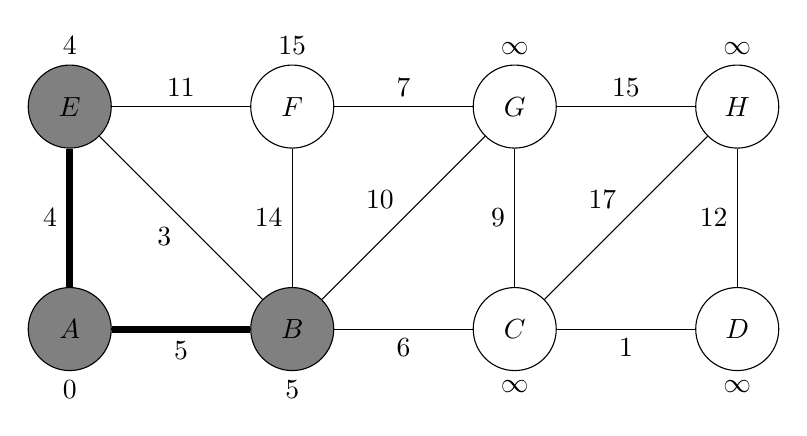
\begin{tikzpicture}[baseline=(E.north), node distance=5em ,c/.style={circle, draw, minimum width=3em}, v/.style={fill=gray}, s/.style={line width=.25em}]
		\node[c, v] (A) {$A$};
		\node[below=0em of A] (A_label) {$0$};
		\node[c, v, right=of A] (B) {$B$};
		\node[below=0em of B] (B_label) {$5$};
		\node[c, right=of B] (C) {$C$};
		\node[below=0em of C] (C_label) {$\infty$};
		\node[c, right=of C] (D) {$D$};
		\node[below=0em of D] (D_label) {$\infty$};
		\node[c, v, above=of A] (E) {$E$};
		\node[above=0em of E] (E_label) {$4$};
		\node[c, above=of B] (F) {$F$};
		\node[above=0em of F] (F_label) {$15$};
		\node[c, above=of C] (G) {$G$};
		\node[above=0em of G] (G_label) {$\infty$};
		\node[c, above=of D] (H) {$H$};
		\node[above=0em of H] (H_label) {$\infty$};

		\path[s] (A) edge node[below] {5} (B);
		\path[s] (A) edge node[auto] {4} (E);
		\path (B) edge node[below] {6} (C);
		\path (B) edge node[auto] {3} (E);
		\path (B) edge node[auto] {14} (F);
		\path (B) edge node[auto] {10} (G);
		\path (C) edge node[below] {1} (D);
		\path (C) edge node[auto] {9} (G);
		\path (C) edge node[auto] {17} (H);
		\path (D) edge node[auto] {12} (H);
		\path (E) edge node[auto] {11} (F);
		\path (F) edge node[auto] {7} (G);
		\path (G) edge node[auto] {15} (H);
	\end{tikzpicture}
	\item
	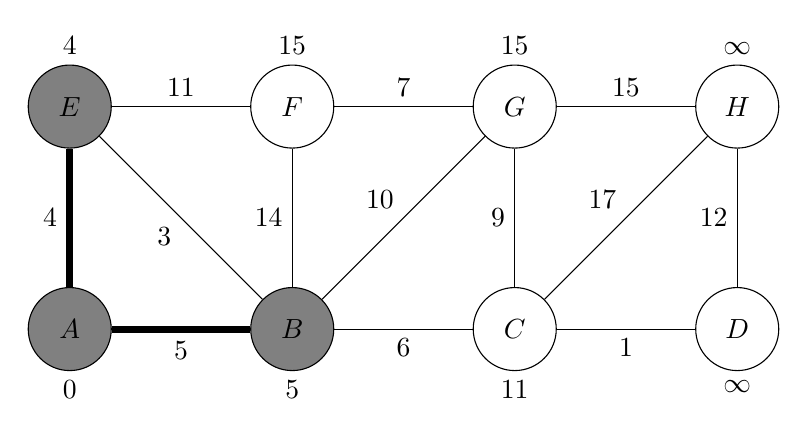
\begin{tikzpicture}[baseline=(E.north), node distance=5em ,c/.style={circle, draw, minimum width=3em}, v/.style={fill=gray}, s/.style={line width=.25em}]
		\node[c, v] (A) {$A$};
		\node[below=0em of A] (A_label) {$0$};
		\node[c, v, right=of A] (B) {$B$};
		\node[below=0em of B] (B_label) {$5$};
		\node[c, right=of B] (C) {$C$};
		\node[below=0em of C] (C_label) {$11$};
		\node[c, right=of C] (D) {$D$};
		\node[below=0em of D] (D_label) {$\infty$};
		\node[c, v, above=of A] (E) {$E$};
		\node[above=0em of E] (E_label) {$4$};
		\node[c, above=of B] (F) {$F$};
		\node[above=0em of F] (F_label) {$15$};
		\node[c, above=of C] (G) {$G$};
		\node[above=0em of G] (G_label) {$15$};
		\node[c, above=of D] (H) {$H$};
		\node[above=0em of H] (H_label) {$\infty$};

		\path[s] (A) edge node[below] {5} (B);
		\path[s] (A) edge node[auto] {4} (E);
		\path (B) edge node[below] {6} (C);
		\path (B) edge node[auto] {3} (E);
		\path (B) edge node[auto] {14} (F);
		\path (B) edge node[auto] {10} (G);
		\path (C) edge node[below] {1} (D);
		\path (C) edge node[auto] {9} (G);
		\path (C) edge node[auto] {17} (H);
		\path (D) edge node[auto] {12} (H);
		\path (E) edge node[auto] {11} (F);
		\path (F) edge node[auto] {7} (G);
		\path (G) edge node[auto] {15} (H);
	\end{tikzpicture}
	\item
	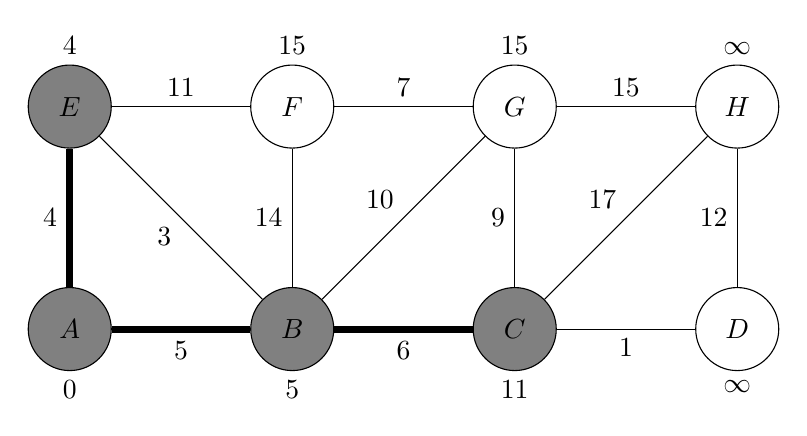
\begin{tikzpicture}[baseline=(E.north), node distance=5em ,c/.style={circle, draw, minimum width=3em}, v/.style={fill=gray}, s/.style={line width=.25em}]
		\node[c, v] (A) {$A$};
		\node[below=0em of A] (A_label) {$0$};
		\node[c, v, right=of A] (B) {$B$};
		\node[below=0em of B] (B_label) {$5$};
		\node[c, v, right=of B] (C) {$C$};
		\node[below=0em of C] (C_label) {$11$};
		\node[c, right=of C] (D) {$D$};
		\node[below=0em of D] (D_label) {$\infty$};
		\node[c, v, above=of A] (E) {$E$};
		\node[above=0em of E] (E_label) {$4$};
		\node[c, above=of B] (F) {$F$};
		\node[above=0em of F] (F_label) {$15$};
		\node[c, above=of C] (G) {$G$};
		\node[above=0em of G] (G_label) {$15$};
		\node[c, above=of D] (H) {$H$};
		\node[above=0em of H] (H_label) {$\infty$};

		\path[s] (A) edge node[below] {5} (B);
		\path[s] (A) edge node[auto] {4} (E);
		\path[s] (B) edge node[below] {6} (C);
		\path (B) edge node[auto] {3} (E);
		\path (B) edge node[auto] {14} (F);
		\path (B) edge node[auto] {10} (G);
		\path (C) edge node[below] {1} (D);
		\path (C) edge node[auto] {9} (G);
		\path (C) edge node[auto] {17} (H);
		\path (D) edge node[auto] {12} (H);
		\path (E) edge node[auto] {11} (F);
		\path (F) edge node[auto] {7} (G);
		\path (G) edge node[auto] {15} (H);
	\end{tikzpicture}
	\item
	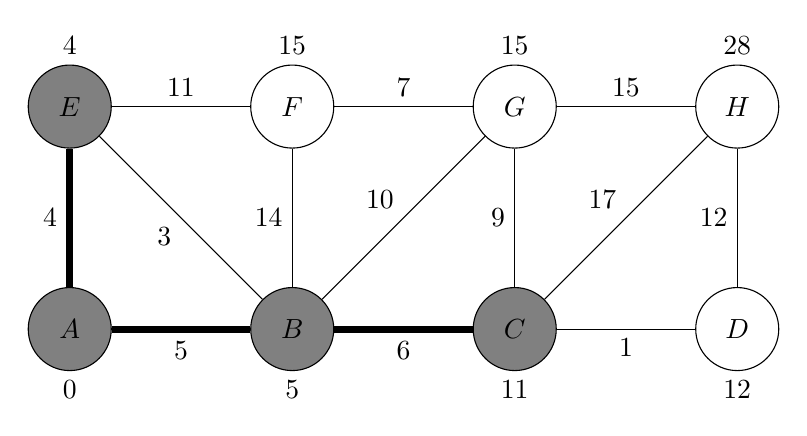
\begin{tikzpicture}[baseline=(E.north), node distance=5em ,c/.style={circle, draw, minimum width=3em}, v/.style={fill=gray}, s/.style={line width=.25em}]
		\node[c, v] (A) {$A$};
		\node[below=0em of A] (A_label) {$0$};
		\node[c, v, right=of A] (B) {$B$};
		\node[below=0em of B] (B_label) {$5$};
		\node[c, v, right=of B] (C) {$C$};
		\node[below=0em of C] (C_label) {$11$};
		\node[c, right=of C] (D) {$D$};
		\node[below=0em of D] (D_label) {$12$};
		\node[c, v, above=of A] (E) {$E$};
		\node[above=0em of E] (E_label) {$4$};
		\node[c, above=of B] (F) {$F$};
		\node[above=0em of F] (F_label) {$15$};
		\node[c, above=of C] (G) {$G$};
		\node[above=0em of G] (G_label) {$15$};
		\node[c, above=of D] (H) {$H$};
		\node[above=0em of H] (H_label) {$28$};

		\path[s] (A) edge node[below] {5} (B);
		\path[s] (A) edge node[auto] {4} (E);
		\path[s] (B) edge node[below] {6} (C);
		\path (B) edge node[auto] {3} (E);
		\path (B) edge node[auto] {14} (F);
		\path (B) edge node[auto] {10} (G);
		\path (C) edge node[below] {1} (D);
		\path (C) edge node[auto] {9} (G);
		\path (C) edge node[auto] {17} (H);
		\path (D) edge node[auto] {12} (H);
		\path (E) edge node[auto] {11} (F);
		\path (F) edge node[auto] {7} (G);
		\path (G) edge node[auto] {15} (H);
	\end{tikzpicture}
	\item
	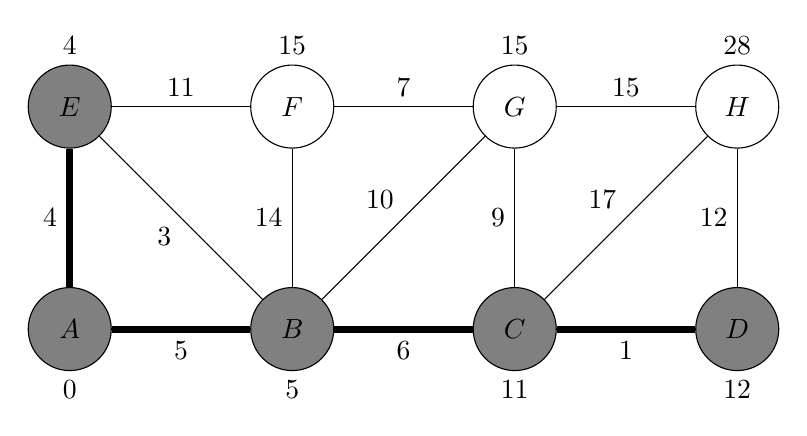
\begin{tikzpicture}[baseline=(E.north), node distance=5em ,c/.style={circle, draw, minimum width=3em}, v/.style={fill=gray}, s/.style={line width=.25em}]
		\node[c, v] (A) {$A$};
		\node[below=0em of A] (A_label) {$0$};
		\node[c, v, right=of A] (B) {$B$};
		\node[below=0em of B] (B_label) {$5$};
		\node[c, v, right=of B] (C) {$C$};
		\node[below=0em of C] (C_label) {$11$};
		\node[c, v, right=of C] (D) {$D$};
		\node[below=0em of D] (D_label) {$12$};
		\node[c, v, above=of A] (E) {$E$};
		\node[above=0em of E] (E_label) {$4$};
		\node[c, above=of B] (F) {$F$};
		\node[above=0em of F] (F_label) {$15$};
		\node[c, above=of C] (G) {$G$};
		\node[above=0em of G] (G_label) {$15$};
		\node[c, above=of D] (H) {$H$};
		\node[above=0em of H] (H_label) {$28$};

		\path[s] (A) edge node[below] {5} (B);
		\path[s] (A) edge node[auto] {4} (E);
		\path[s] (B) edge node[below] {6} (C);
		\path (B) edge node[auto] {3} (E);
		\path (B) edge node[auto] {14} (F);
		\path (B) edge node[auto] {10} (G);
		\path[s] (C) edge node[below] {1} (D);
		\path (C) edge node[auto] {9} (G);
		\path (C) edge node[auto] {17} (H);
		\path (D) edge node[auto] {12} (H);
		\path (E) edge node[auto] {11} (F);
		\path (F) edge node[auto] {7} (G);
		\path (G) edge node[auto] {15} (H);
	\end{tikzpicture}
	\item
	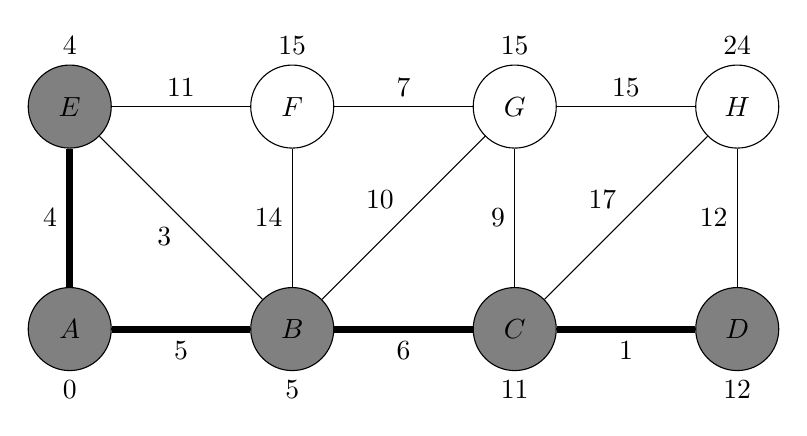
\begin{tikzpicture}[baseline=(E.north), node distance=5em ,c/.style={circle, draw, minimum width=3em}, v/.style={fill=gray}, s/.style={line width=.25em}]
		\node[c, v] (A) {$A$};
		\node[below=0em of A] (A_label) {$0$};
		\node[c, v, right=of A] (B) {$B$};
		\node[below=0em of B] (B_label) {$5$};
		\node[c, v, right=of B] (C) {$C$};
		\node[below=0em of C] (C_label) {$11$};
		\node[c, v, right=of C] (D) {$D$};
		\node[below=0em of D] (D_label) {$12$};
		\node[c, v, above=of A] (E) {$E$};
		\node[above=0em of E] (E_label) {$4$};
		\node[c, above=of B] (F) {$F$};
		\node[above=0em of F] (F_label) {$15$};
		\node[c, above=of C] (G) {$G$};
		\node[above=0em of G] (G_label) {$15$};
		\node[c, above=of D] (H) {$H$};
		\node[above=0em of H] (H_label) {$24$};

		\path[s] (A) edge node[below] {5} (B);
		\path[s] (A) edge node[auto] {4} (E);
		\path[s] (B) edge node[below] {6} (C);
		\path (B) edge node[auto] {3} (E);
		\path (B) edge node[auto] {14} (F);
		\path (B) edge node[auto] {10} (G);
		\path[s] (C) edge node[below] {1} (D);
		\path (C) edge node[auto] {9} (G);
		\path (C) edge node[auto] {17} (H);
		\path (D) edge node[auto] {12} (H);
		\path (E) edge node[auto] {11} (F);
		\path (F) edge node[auto] {7} (G);
		\path (G) edge node[auto] {15} (H);
	\end{tikzpicture}
	\item
	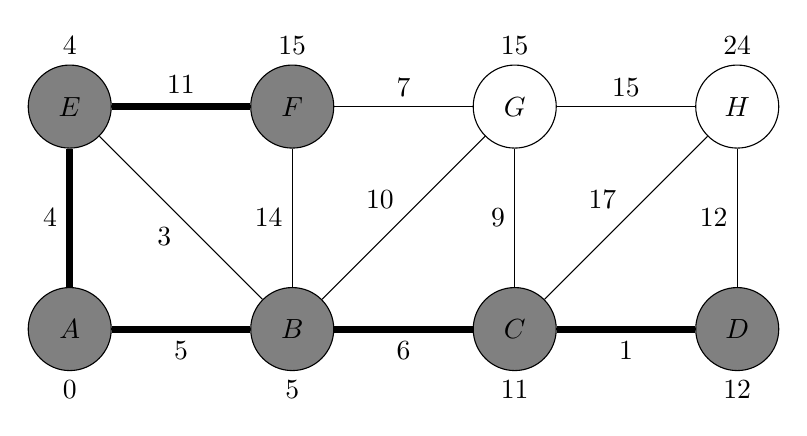
\begin{tikzpicture}[baseline=(E.north), node distance=5em ,c/.style={circle, draw, minimum width=3em}, v/.style={fill=gray}, s/.style={line width=.25em}]
		\node[c, v] (A) {$A$};
		\node[below=0em of A] (A_label) {$0$};
		\node[c, v, right=of A] (B) {$B$};
		\node[below=0em of B] (B_label) {$5$};
		\node[c, v, right=of B] (C) {$C$};
		\node[below=0em of C] (C_label) {$11$};
		\node[c, v, right=of C] (D) {$D$};
		\node[below=0em of D] (D_label) {$12$};
		\node[c, v, above=of A] (E) {$E$};
		\node[above=0em of E] (E_label) {$4$};
		\node[c, v, above=of B] (F) {$F$};
		\node[above=0em of F] (F_label) {$15$};
		\node[c, above=of C] (G) {$G$};
		\node[above=0em of G] (G_label) {$15$};
		\node[c, above=of D] (H) {$H$};
		\node[above=0em of H] (H_label) {$24$};

		\path[s] (A) edge node[below] {5} (B);
		\path[s] (A) edge node[auto] {4} (E);
		\path[s] (B) edge node[below] {6} (C);
		\path (B) edge node[auto] {3} (E);
		\path (B) edge node[auto] {14} (F);
		\path (B) edge node[auto] {10} (G);
		\path[s] (C) edge node[below] {1} (D);
		\path (C) edge node[auto] {9} (G);
		\path (C) edge node[auto] {17} (H);
		\path (D) edge node[auto] {12} (H);
		\path[s] (E) edge node[auto] {11} (F);
		\path (F) edge node[auto] {7} (G);
		\path (G) edge node[auto] {15} (H);
	\end{tikzpicture}
	\item
	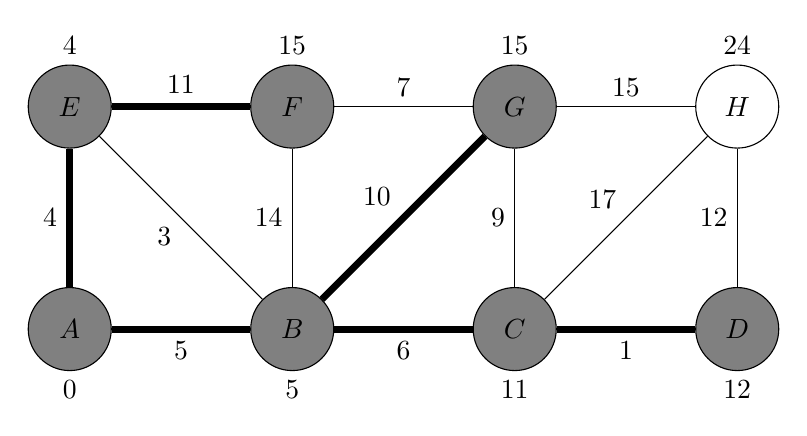
\begin{tikzpicture}[baseline=(E.north), node distance=5em ,c/.style={circle, draw, minimum width=3em}, v/.style={fill=gray}, s/.style={line width=.25em}]
		\node[c, v] (A) {$A$};
		\node[below=0em of A] (A_label) {$0$};
		\node[c, v, right=of A] (B) {$B$};
		\node[below=0em of B] (B_label) {$5$};
		\node[c, v, right=of B] (C) {$C$};
		\node[below=0em of C] (C_label) {$11$};
		\node[c, v, right=of C] (D) {$D$};
		\node[below=0em of D] (D_label) {$12$};
		\node[c, v, above=of A] (E) {$E$};
		\node[above=0em of E] (E_label) {$4$};
		\node[c, v, above=of B] (F) {$F$};
		\node[above=0em of F] (F_label) {$15$};
		\node[c, v, above=of C] (G) {$G$};
		\node[above=0em of G] (G_label) {$15$};
		\node[c, above=of D] (H) {$H$};
		\node[above=0em of H] (H_label) {$24$};

		\path[s] (A) edge node[below] {5} (B);
		\path[s] (A) edge node[auto] {4} (E);
		\path[s] (B) edge node[below] {6} (C);
		\path (B) edge node[auto] {3} (E);
		\path (B) edge node[auto] {14} (F);
		\path[s] (B) edge node[auto] {10} (G);
		\path[s] (C) edge node[below] {1} (D);
		\path (C) edge node[auto] {9} (G);
		\path (C) edge node[auto] {17} (H);
		\path (D) edge node[auto] {12} (H);
		\path[s] (E) edge node[auto] {11} (F);
		\path (F) edge node[auto] {7} (G);
		\path (G) edge node[auto] {15} (H);
	\end{tikzpicture}
	\item
	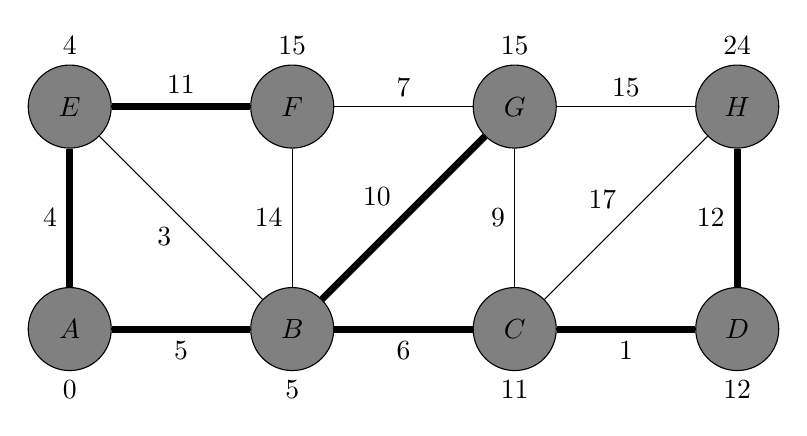
\begin{tikzpicture}[baseline=(E.north), node distance=5em ,c/.style={circle, draw, minimum width=3em}, v/.style={fill=gray}, s/.style={line width=.25em}]
		\node[c, v] (A) {$A$};
		\node[below=0em of A] (A_label) {$0$};
		\node[c, v, right=of A] (B) {$B$};
		\node[below=0em of B] (B_label) {$5$};
		\node[c, v, right=of B] (C) {$C$};
		\node[below=0em of C] (C_label) {$11$};
		\node[c, v, right=of C] (D) {$D$};
		\node[below=0em of D] (D_label) {$12$};
		\node[c, v, above=of A] (E) {$E$};
		\node[above=0em of E] (E_label) {$4$};
		\node[c, v, above=of B] (F) {$F$};
		\node[above=0em of F] (F_label) {$15$};
		\node[c, v, above=of C] (G) {$G$};
		\node[above=0em of G] (G_label) {$15$};
		\node[c, v, above=of D] (H) {$H$};
		\node[above=0em of H] (H_label) {$24$};

		\path[s] (A) edge node[below] {5} (B);
		\path[s] (A) edge node[auto] {4} (E);
		\path[s] (B) edge node[below] {6} (C);
		\path (B) edge node[auto] {3} (E);
		\path (B) edge node[auto] {14} (F);
		\path[s] (B) edge node[auto] {10} (G);
		\path[s] (C) edge node[below] {1} (D);
		\path (C) edge node[auto] {9} (G);
		\path (C) edge node[auto] {17} (H);
		\path[s] (D) edge node[auto] {12} (H);
		\path[s] (E) edge node[auto] {11} (F);
		\path (F) edge node[auto] {7} (G);
		\path (G) edge node[auto] {15} (H);
	\end{tikzpicture}
\end{enumerate}

Nodes in exploration order: $\{A, E, B, C, D, F, G, H\}$.

\section{} %3
Dijkstra's algorithm produces wrong output for some graphs with negatively weighted edges such as this one:

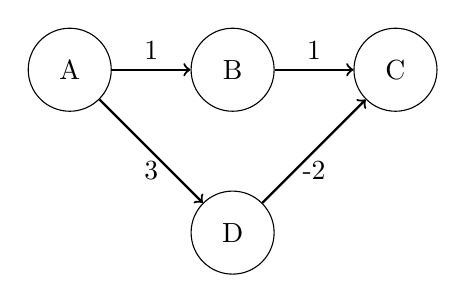
\begin{tikzpicture}[c/.style={circle, draw, minimum width=3em}]
	\node[c] (A) {A};
	\node[c, right=of A] (B) {B};
	\node[c, right=of B] (C) {C};
	\node[c, below=of B] (D) {D};

	\path[->, thick] (A) edge node[above] {1} (B);
	\path[->, thick] (A) edge node[below] {3} (D);
	\path[->, thick] (B) edge node[above] {1} (C);
	\path[->, thick] (D) edge node[below] {-2} (C);
\end{tikzpicture}

When we run Dijkstra's algorithm:

\begin{enumerate}
	\item
	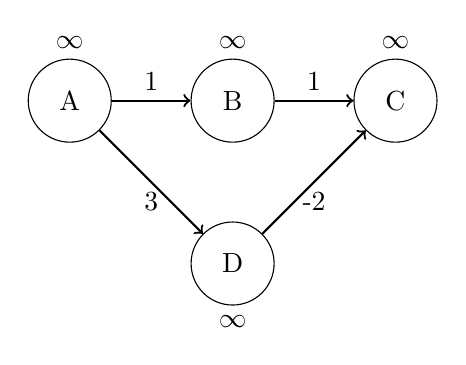
\begin{tikzpicture}[baseline=(A.north), c/.style={circle, draw, minimum width=3em}, v/.style={fill=gray}]
		\node[c] (A) {A};
		\node[above=0em of A] (A_label) {$\infty$};
		\node[c, right=of A] (B) {B};
		\node[above=0em of B] (B_label) {$\infty$};
		\node[c, right=of B] (C) {C};
		\node[above=0em of C] (C_label) {$\infty$};
		\node[c, below=of B] (D) {D};
		\node[below=0em of D] (D_label) {$\infty$};


		\path[->, thick] (A) edge node[above] {1} (B);
		\path[->, thick] (A) edge node[below] {3} (D);
		\path[->, thick] (B) edge node[above] {1} (C);
		\path[->, thick] (D) edge node[below] {-2} (C);
	\end{tikzpicture}
	\item
	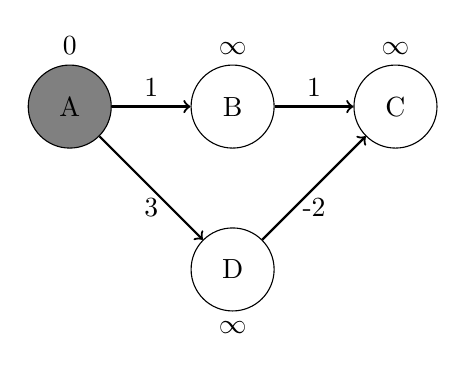
\begin{tikzpicture}[baseline=(A.north), c/.style={circle, draw, minimum width=3em}, v/.style={fill=gray}]
		\node[c, v] (A) {A};
		\node[above=0em of A] (A_label) {$0$};
		\node[c, right=of A] (B) {B};
		\node[above=0em of B] (B_label) {$\infty$};
		\node[c, right=of B] (C) {C};
		\node[above=0em of C] (C_label) {$\infty$};
		\node[c, below=of B] (D) {D};
		\node[below=0em of D] (D_label) {$\infty$};


		\path[->, thick] (A) edge node[above] {1} (B);
		\path[->, thick] (A) edge node[below] {3} (D);
		\path[->, thick] (B) edge node[above] {1} (C);
		\path[->, thick] (D) edge node[below] {-2} (C);
	\end{tikzpicture}
	\item
	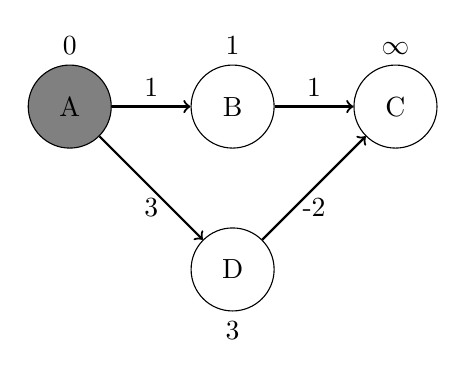
\begin{tikzpicture}[baseline=(A.north), c/.style={circle, draw, minimum width=3em}, v/.style={fill=gray}]
		\node[c, v] (A) {A};
		\node[above=0em of A] (A_label) {$0$};
		\node[c, right=of A] (B) {B};
		\node[above=0em of B] (B_label) {$1$};
		\node[c, right=of B] (C) {C};
		\node[above=0em of C] (C_label) {$\infty$};
		\node[c, below=of B] (D) {D};
		\node[below=0em of D] (D_label) {$3$};


		\path[->, thick] (A) edge node[above] {1} (B);
		\path[->, thick] (A) edge node[below] {3} (D);
		\path[->, thick] (B) edge node[above] {1} (C);
		\path[->, thick] (D) edge node[below] {-2} (C);
	\end{tikzpicture}
	\item
	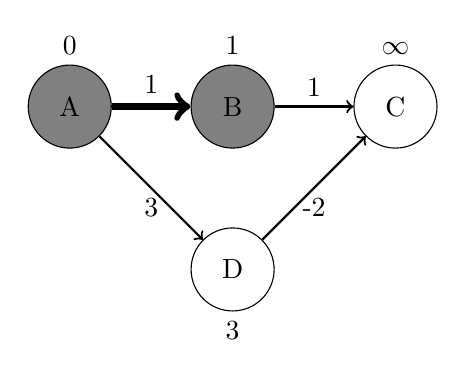
\begin{tikzpicture}[baseline=(A.north), c/.style={circle, draw, minimum width=3em}, v/.style={fill=gray}, s/.style={line width=.25em}]
		\node[c, v] (A) {A};
		\node[above=0em of A] (A_label) {$0$};
		\node[c, v, right=of A] (B) {B};
		\node[above=0em of B] (B_label) {$1$};
		\node[c, right=of B] (C) {C};
		\node[above=0em of C] (C_label) {$\infty$};
		\node[c, below=of B] (D) {D};
		\node[below=0em of D] (D_label) {$3$};


		\path[->, thick, s] (A) edge node[above] {1} (B);
		\path[->, thick] (A) edge node[below] {3} (D);
		\path[->, thick] (B) edge node[above] {1} (C);
		\path[->, thick] (D) edge node[below] {-2} (C);
	\end{tikzpicture}
	\item
	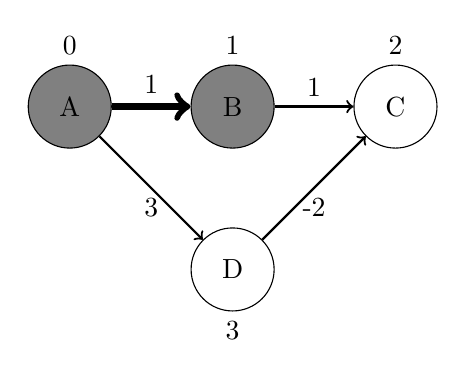
\begin{tikzpicture}[baseline=(A.north), c/.style={circle, draw, minimum width=3em}, v/.style={fill=gray}, s/.style={line width=.25em}]
		\node[c, v] (A) {A};
		\node[above=0em of A] (A_label) {$0$};
		\node[c, v, right=of A] (B) {B};
		\node[above=0em of B] (B_label) {$1$};
		\node[c, right=of B] (C) {C};
		\node[above=0em of C] (C_label) {$2$};
		\node[c, below=of B] (D) {D};
		\node[below=0em of D] (D_label) {$3$};


		\path[->, thick, s] (A) edge node[above] {1} (B);
		\path[->, thick] (A) edge node[below] {3} (D);
		\path[->, thick] (B) edge node[above] {1} (C);
		\path[->, thick] (D) edge node[below] {-2} (C);
	\end{tikzpicture}
	\item
	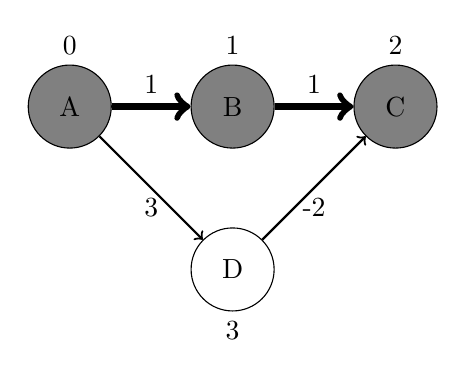
\begin{tikzpicture}[baseline=(A.north), c/.style={circle, draw, minimum width=3em}, v/.style={fill=gray}, s/.style={line width=.25em}]
		\node[c, v] (A) {A};
		\node[above=0em of A] (A_label) {$0$};
		\node[c, v, right=of A] (B) {B};
		\node[above=0em of B] (B_label) {$1$};
		\node[c, v, right=of B] (C) {C};
		\node[above=0em of C] (C_label) {$2$};
		\node[c, below=of B] (D) {D};
		\node[below=0em of D] (D_label) {$3$};


		\path[->, thick, s] (A) edge node[above] {1} (B);
		\path[->, thick] (A) edge node[below] {3} (D);
		\path[->, thick, s] (B) edge node[above] {1} (C);
		\path[->, thick] (D) edge node[below] {-2} (C);
	\end{tikzpicture}
	\item
	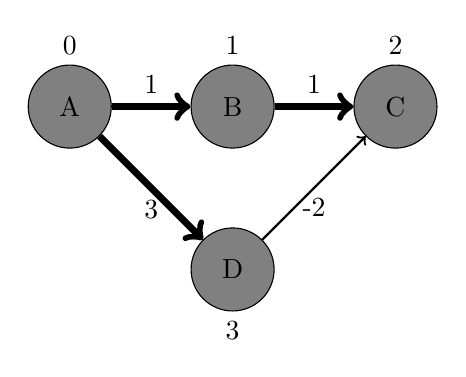
\begin{tikzpicture}[baseline=(A.north), c/.style={circle, draw, minimum width=3em}, v/.style={fill=gray}, s/.style={line width=.25em}]
		\node[c, v] (A) {A};
		\node[above=0em of A] (A_label) {$0$};
		\node[c, v, right=of A] (B) {B};
		\node[above=0em of B] (B_label) {$1$};
		\node[c, v, right=of B] (C) {C};
		\node[above=0em of C] (C_label) {$2$};
		\node[c, v, below=of B] (D) {D};
		\node[below=0em of D] (D_label) {$3$};


		\path[->, thick, s] (A) edge node[above] {1} (B);
		\path[->, thick, s] (A) edge node[below] {3} (D);
		\path[->, thick, s] (B) edge node[above] {1} (C);
		\path[->, thick] (D) edge node[below] {-2} (C);
	\end{tikzpicture}
\end{enumerate}

The shortest path it finds is $((A, B), (B, C))$ which is of length $2$ while $((A, D), (D, C))$ is of length $1$. This is because the algorithm assumes that path lengths are monotonically increasing. This allows it to further assume that by being greedy it finds the shortest paths. By giving edges negative weights we violate that property and the algorithms fails to find the shortest path.

\section{} %4
I a max-heap the smallest element may reside inside a leaf node. This can be proven by a property of the heap: "If node $A$ is a parent of node $B$ then the value of $A$ is ordered with respect to the value of node B with the same ordering applying across the whole heap.". For a max-heap this ordering is $A > B$.

\begin{enumerate}
	\item \label{q4:a_is_smallest}
	We look at any non-leaf node $A$ and assume it contains the smallest element in the heap.
	\item \label{q4:b_is_smaller}
	According to our heap property child $B$ of node $A$ contains a smaller value than $A$.
	\item
	(\ref{q4:b_is_smaller}) and (\ref{q4:a_is_smallest}) contradict each other.
\end{enumerate}

By assuming that any non-leaf node contains the smallest element we get a contradiction the smallest value may only reside inside a leaf node.

\section{} %5
We want to find the shortest path from $u$ to $v$ that passes through $v_0$.

First we perform Dijkstra's algorithm to find the shortest paths between all nodes. The shortest path from $u$ to $v$ passing through $v_0$ is $(u, v_0) + (v_0, v)$. Dijkstra's algorithm already gave us $(u, v_0)$ and $(v_0, v)$.

\section{} %6
Making all edge's weights non-negative by adding a constant to all edges is a valid method. This makes distances monotonically increasing. Dijksta's algorithm is greedy and always explores the node with the lowest distance.

We have out invariants:
\begin{itemize}
	\item $dist(A)$ is the shortest path from start $S$ to $A$ for each visited node $A$.
	\item $dist(X)$ is the shortest path from $S$ to $X$ we know of, for each unvisited node $X$.
\end{itemize}

With just one visited node they are obviously true.

We also assume this for $k$ visited nodes and choose the unvisited node $X$ for which $dist(X)$ is minimal (greedy) and $dist(X) = dist(A) + weight((A, X))$. $dist(X)$ must be minimal as if there were a shorter path to $X$ via another unvisited node $Y$ then $dist(Y)$ would need to be less than $dist(X)$ because the distance is monotonically increasing. This cannot be true according to our invariants because if $dist(Y) < dist(X)$ then $Y$ is explored before $X$.

\end{document}
